\section{Real-time Evaluation and Model Benchmarking}
\label{sec:integrating}

This section details the deployment of the quantized YOLO-MobileNetV4 model onto an AUTOSAR Adaptive Platform. The integration process involves establishing a toolchain for service-oriented architecture configuration, designing the system topology, and evaluating the inference performance on the target edge device unit.

% \subsection{Toolchains and Workflow}
% Leveraging the PopcornSAR ecosystem introduced in Section \ref{sec:related_work}, we adopted a Model-Based Development (MBD) workflow using the \textit{AutoSAR.io} authoring tool and Para-SDK. The development process is divided into three key stages:

% \begin{enumerate}
%     \item \textit{System Configuration:} We utilized \textit{AutoSAR.io} to model the Adaptive Application (AA) architecture. This involved defining the Service Interfaces for the camera sensor (Provider) and visualization unit (Consumer), configuring Events for high-bandwidth video transmission, and mapping these software components to the specific Machine Manifest representing the target hardware.
    
%     \item \textit{Code Generation:} From the configured \texttt{.arxml} descriptions, the Para-Generator automatically produced the C++ Service Interface Skeletons and Proxies. This step abstracts the complexity of the underlying SOME/IP communication protocol, ensuring compliance with the AUTOSAR standard.
    
%     \item \textit{Integration and Implementation:} The generated C++ artifacts were integrated with the Para-SDK middleware libraries (\texttt{libara}). Within this environment, we embedded the TFLite runtime engine into the Execution Management lifecycle, enabling the application to handle real-time inference while managing service-oriented communication via the Communication Management API.
% \end{enumerate}

\subsection{Toolchains and Workflow Configuration}
Leveraging the PopcornSAR ecosystem introduced in Section \ref{sec:related_work}, the system was implemented following a model-based development workflow. System modeling and service configuration were performed using the \textit{AutoSAR.io} authoring tool, while application development and runtime support relied on the \textit{PARA SDK}.

At a high level, the workflow consists of three main steps. First, the Adaptive Application architecture and service interfaces were defined in \textit{AutoSAR.io}, including provider--consumer relationships for camera input and perception output, as well as event-based communication over SOME/IP \cite{autosar_someip_r21_11}. Second, the configured \texttt{.arxml} descriptions were used to automatically generate C++ service skeletons and proxies, ensuring compliance with AUTOSAR communication standards. Finally, the generated artifacts were integrated with the PARA SDK runtime libraries, where the LiteRT inference engine was embedded into the application lifecycle to enable real-time perception within a service-oriented execution environment. Based on the configured toolchain and model-based workflow, our proposed approach will be presented.


\subsection{Proposed Approach}
The proposed approach, illustrated in Figure ~\ref{fig:arch_design}, follows a Producer-Consumer communication pattern implemented via SOME/IP \cite{autosar_someip_r21_11} and is designed around an edge AI–centric sensing paradigm.

\begin{figure}[htbp]
    \centering
    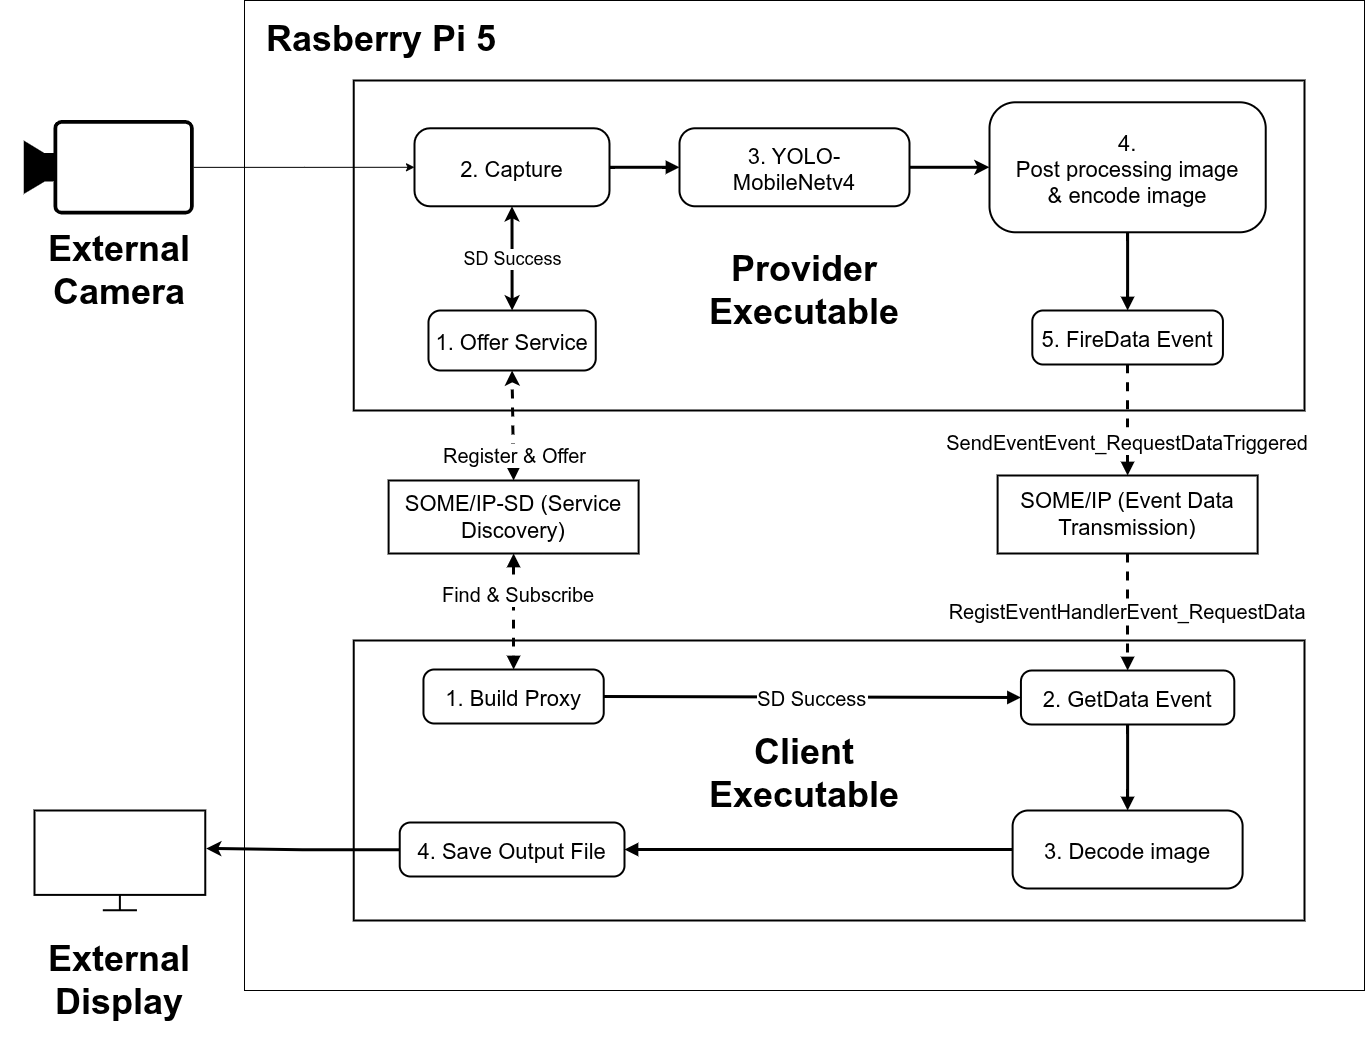
\includegraphics[width=1\linewidth]{Images/sysArch.png}
    \caption{Proposed approach of the AUTOSAR Adaptive Platform Traffic Light Detection System on Rasberry Pi 5.}
    \label{fig:arch_design}
\end{figure}

The system consists of two Adaptive AUTOSAR Applications deployed on the edge device, where intelligence is pushed directly to the sensor node to minimize data transmission and latency:

\begin{itemize}
    \item \textit{Provider Executable (Send):} Interfacing directly with an external camera, this edge node executes a five-stage pipeline: (1) offering the service via SOME/IP-SD; (2) capturing live video frames; (3) performing real-time YOLO-MobileNetV4 inference; (4) post-processing the annotated image and encoding it into a vector; and (5) triggering a data event (\texttt{SendEvent\_RequestDataTriggered}) to transmit the vector data.

    \item \textit{Client Executable (Receive):} Acting as the service consumer, it reconstructs the transmitted data by: (1) finding the service and building a proxy via SOME/IP-SD; (2) handling the received data event (\texttt{RegistEventHandler\_RequestData}); (3) decoding the vector into a image; and (4) saving the output for external display rendering.

    \item \textit{SOME/IP Communication:} This middleware manages dynamic service registration and discovery via SOME/IP-SD. To handle the transmission of heavy encoded image payloads, the SOME/IP Transport Protocol (SOME/IP-TP) is utilized to segment and reassemble large messages across the network.
\end{itemize}

To validate the effectiveness of the proposed architecture, the following section evaluates the system's real-time performance and detection quality on the embedded edge device.

\subsection{Dataset and Training Setup}

To evaluate our object detection models, we created a dataset named \textit{Traffic Lights}, which contains 6,536 images and 9,738 annotated traffic light instances under diverse, real-world conditions. The dataset was partitioned into training (5,712 images, 87.4\%), validation (548 images, 8.4\%), and testing (276 images, 4.2\%) sets, with no empty frames. Annotations are categorized into three classes exhibiting a natural imbalance: Green (50.3\%), Red (35.0\%), and a minority Yellow class (14.7\%).

During preprocessing, all images were resized to $320 \times 320$ pixels and normalized to the $[0, 1]$ range. To mitigate the class imbalance and enhance model generalization, we applied Mosaic data augmentation during training. This technique combines four distinct images into a single frame to simulate varying object scales and partial occlusions. 

All experiments were conducted on a Windows 11 workstation. The software environment was isolated using a Python virtual environment (\texttt{venv}), and model training was accelerated using an NVIDIA GeForce RTX 4060 8GB GPU.

% \subsection{Dataset and Training Setup}

% To train and evaluate the proposed object detection models, we utilized the \textit{Traffic Light.v1i.yolo26} dataset, which was specifically selected for its diverse capture conditions representative of real-world traffic scenarios. The dataset comprises a total of 6,536 images and yields 9,738 annotated traffic light instances, with no empty frames present in the collection. To ensure robust model training and evaluation, the data was partitioned into training, validation, and testing sets, as detailed in Table \ref{tab:dataset_splits}. 

% \begin{table}[ht]
% \centering
% \caption{Dataset Partition Details}
% \label{tab:dataset_splits}
% \resizebox{\columnwidth}{!}{
% \renewcommand{\arraystretch}{1.3}
% \begin{tabular}{|l|c|c|c|}
% \hline
% Split & Images & Percentage & Instances \\ \hline
% Training & 5,712 & 87.4\% & 8,564 \\ \hline
% Validation & 548 & 8.4\% & 742 \\ \hline
% Testing & 276 & 4.2\% & 432 \\ \hline
% Total & 6,536 & 100.0\% & 9,738 \\ \hline
% \end{tabular}
% }
% \end{table}

% The dataset annotations are categorized into three primary traffic light states: Green, Red, and Yellow. An analysis of the class distribution across the entire dataset reveals a natural class imbalance inherent to standard traffic light cycles. As shown in Table \ref{tab:class_dist}, the Green class constitutes the majority, while the Yellow class represents a significant minority. 

% \begin{table}[ht]
% \centering
% \caption{Class Distribution Across Dataset Splits}
% \label{tab:class_dist}
% \resizebox{\columnwidth}{!}{
% \renewcommand{\arraystretch}{1.3}
% \begin{tabular}{|l|c|c|c|l|}
% \hline
% Class & Training & Validation & Testing & Total (\%) \\ \hline
% Green & 4,265 & 395 & 241 & 4,901 (50.3\%) \\ \hline
% Red & 3,047 & 221 & 138 & 3,406 (35.0\%) \\ \hline
% Yellow & 1,252 & 126 & 53 & 1,431 (14.7\%) \\ \hline
% \end{tabular}
% }
% \end{table}

% For preprocessing, all input images were resized to 320x320 pixels and normalized to the [0, 1] range. To prevent overfitting and mitigate the observed class imbalance, we applied Mosaic data augmentation during training. By combining four distinct images into a single frame, this technique simulates varying object scales and partial occlusions, ultimately improving the model's generalization in complex traffic environments.

% All experiments and model training were conducted on a workstation running Windows 11. To ensure dependency isolation and reproducibility, the software environment was managed using a Python virtual environment (\texttt{venv}). The computational demands of training the network were handled utilizing an NVIDIA GeForce RTX 4060 as the primary hardware accelerator.

\subsection{Compared Models}
To analyze the speed-accuracy trade-off for embedded traffic light detection, four models were evaluated: YOLO11n, YOLO11-MobileNetV4 (ConvSmall), YOLO8n, and SSD-MobileNetV3.

\subsubsection{Detection Accuracy} 

As detailed in Table~\ref{tab:tradeoff_yolo_models}, the standard YOLO architectures (YOLO11n, YOLO8n) achieve the highest detection accuracies, all exceeding 0.97 in mAP@50. Replacing the backbone with MobileNetV4 in YOLO11 results in an expected accuracy trade-off, reducing the mAP@50 from 0.977 to 0.929 (a relative decrease of approximately 4.9\%). However, YOLO11-MobileNetV4 still outperforms the traditional SSD-MobileNetV3 baseline (mAP@50 of 0.743), demonstrating sufficient detection performance for the targeted traffic light recognition task.

\subsubsection{Inference Speed}

Inference latency is the primary bottleneck for edge deployment. According to the experimental results summarized in Table~\ref{tab:tradeoff_yolo_models}, the original YOLO11n in LiteRT format requires approximately 90\,ms per frame. While older architectures like YOLO8n improve this to roughly 78\,ms, the YOLO11-MobileNetV4 model significantly reduces inference latency to approximately 38\,ms. 

This represents a $\sim$2.4$\times$ speedup (an approximately 58\% reduction in latency) compared to the baseline YOLO11n. Furthermore, it achieves a faster inference time than the SSD-MobileNetV3 model ($\sim$44\,ms) while maintaining a notably higher mAP@50 (0.929 vs. 0.743). This latency reduction enables real-time performance of approximately 26 FPS on embedded hardware, validating the suitability of the MobileNetV4 backbone for real-time edge inference.

\begin{table}[ht]
\centering
\caption{Performance trade-off between Different Models}
\label{tab:tradeoff_yolo_models}
\resizebox{\columnwidth}{!}{
\renewcommand{\arraystretch}{1.3}
\begin{tabular}{|l|l|c|c|l|}
\hline
Model & Format & mAP@50 (\%) & mAP@50-95 (\%) & Inference Time \\ \hline
YOLO11n & LiteRT & \textbf{97.7} & 78.5 & $\sim$90ms \\ \hline
\begin{tabular}[c]{@{}l@{}}YOLO11n-MobileNetV4 \\ (Ours)\end{tabular} & LiteRT & 92.9 & 72.3 & \textbf{$\sim$38ms} \\ \hline
YOLO8n & LiteRT & 97.4 & \textbf{81.1} & $\sim$78ms \\ \hline
SSD-MobilenetV3 & ONNX & 74.3 & 54.8 & $\sim$44ms \\ \hline
\end{tabular}
}
\end{table}

The experimental results demonstrate the feasibility and efficiency of the proposed approach for real-time traffic light detection on edge devices. Based on these findings, the final section summarizes the key contributions and discusses the implications for future AUTOSAR-based edge perception systems.

\subsection{Result and Evaluation}
% 0305667542 As described in Section~\ref{sec:comparison}, the system was evaluated in terms of inference accuracy and real-time performance using a C++ Adaptive AUTOSAR implementation deployed on a Raspberry Pi~5 (without TPU/GPU and SSD storage). This setup represents a cost-effective embedded edge platform relying solely on CPU-based inference.

The system was evaluated in terms of inference accuracy and real-time performance using a C++ Adaptive AUTOSAR implementation deployed on the above Deployment Setup.
\begin{figure}[htbp]
    \centering
    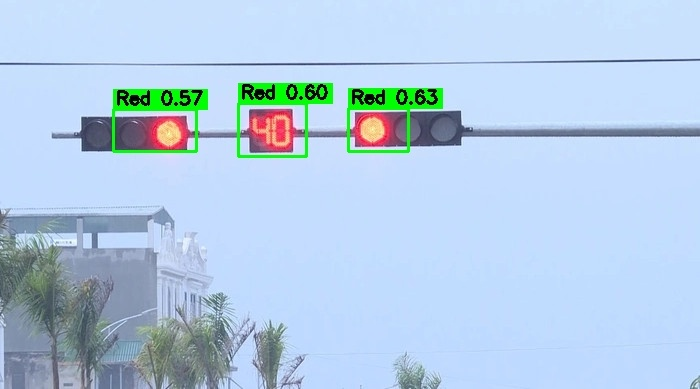
\includegraphics[width=1\linewidth]{Images/received_output.jpg}
    \caption{Traffic light detection results on YOLO11-MobileNetV4 model using the proposed AUTOSAR Adaptive Platform C++ implementation on a Raspberry Pi 5.}
    \label{fig:res_cpp}
\end{figure}

% As shown in Fig.~\ref{fig:res_cpp}, the proposed system successfully detects traffic lights with accurate bounding box localization and correct class prediction (e.g., \textit{Red}). These qualitative results confirm that the integration of the LiteRT inference runtime within the Adaptive AUTOSAR framework operates correctly on embedded hardware without observable degradation in detection quality.

% Key performance metrics obtained from runtime logs include:
% \begin{itemize}
%     \item \textit{Confidence Scores:} The system consistently reports stable detection confidence values (e.g., 0.63 for the rightmost traffic signal), indicating effective quantization and model integration.
%     \item \textit{Inference Latency:} Pure CPU execution achieves an average inference time of approximately 36\,ms per frame (as evidenced by the log output: \textit{``Inference time: 29.9893 ms''}).
%     \item \textit{End-to-End Latency:} Including pre-processing, inference, post-processing, and SOME/IP message preparation, the total latency averages around 41\,ms, supporting real-time operation at approximately 24--25\,FPS.
% \end{itemize}

% These results demonstrate that real-time traffic light detection can be achieved within a standardized Adaptive AUTOSAR architecture using low-cost, CPU-based embedded hardware, without reliance on dedicated AI accelerators. This highlights the feasibility of deploying scalable and cost-efficient perception services in automotive edge systems. 

% While the qualitative and runtime results confirm the feasibility of the proposed system, a quantitative comparison with alternative model configurations is necessary to analyze the speed-accuracy trade-off for embedded deployment.

As shown in Fig.~\ref{fig:res_cpp}, the proposed system successfully detects traffic lights with accurate bounding box localization and correct class prediction (e.g., \textit{Red}). Key performance metrics obtained from runtime logs reveal that the system consistently reports stable detection confidence values, such as 0.63 for the rightmost traffic signal. These qualitative results confirm that the integration of the LiteRT inference runtime within the Adaptive AUTOSAR framework operates correctly on embedded hardware, indicating effective quantization and model integration without observable degradation in detection quality.

These findings demonstrate that real-time traffic light detection can be successfully achieved within a standardized Adaptive AUTOSAR architecture using low-cost, CPU-based embedded hardware, entirely without reliance on dedicated AI accelerators. This highlights the broader feasibility of deploying scalable and cost-efficient perception services directly into automotive edge systems. While the qualitative and runtime results confirm the operational feasibility of the proposed system, a comprehensive evaluation requires further context. Therefore, a quantitative comparison with alternative model configurations is necessary to thoroughly analyze the speed-accuracy trade-off for optimal embedded deployment.


% \subsection{Compared Models}
% The models were evaluated to analyze the speed--accuracy trade-off for embedded traffic light detection:
% \begin{itemize}
%     \item YOLO11n
%     \item YOLO11n--MobileNetV4 (ConvSmall)
%     \item YOLO8n
%     \item YOLO26n
%     \item SSD-MobileNetV3
% \end{itemize}
% \subsubsection{Detection Accuracy} 

% % \begin{figure}[ht]
% %     \centering
% %     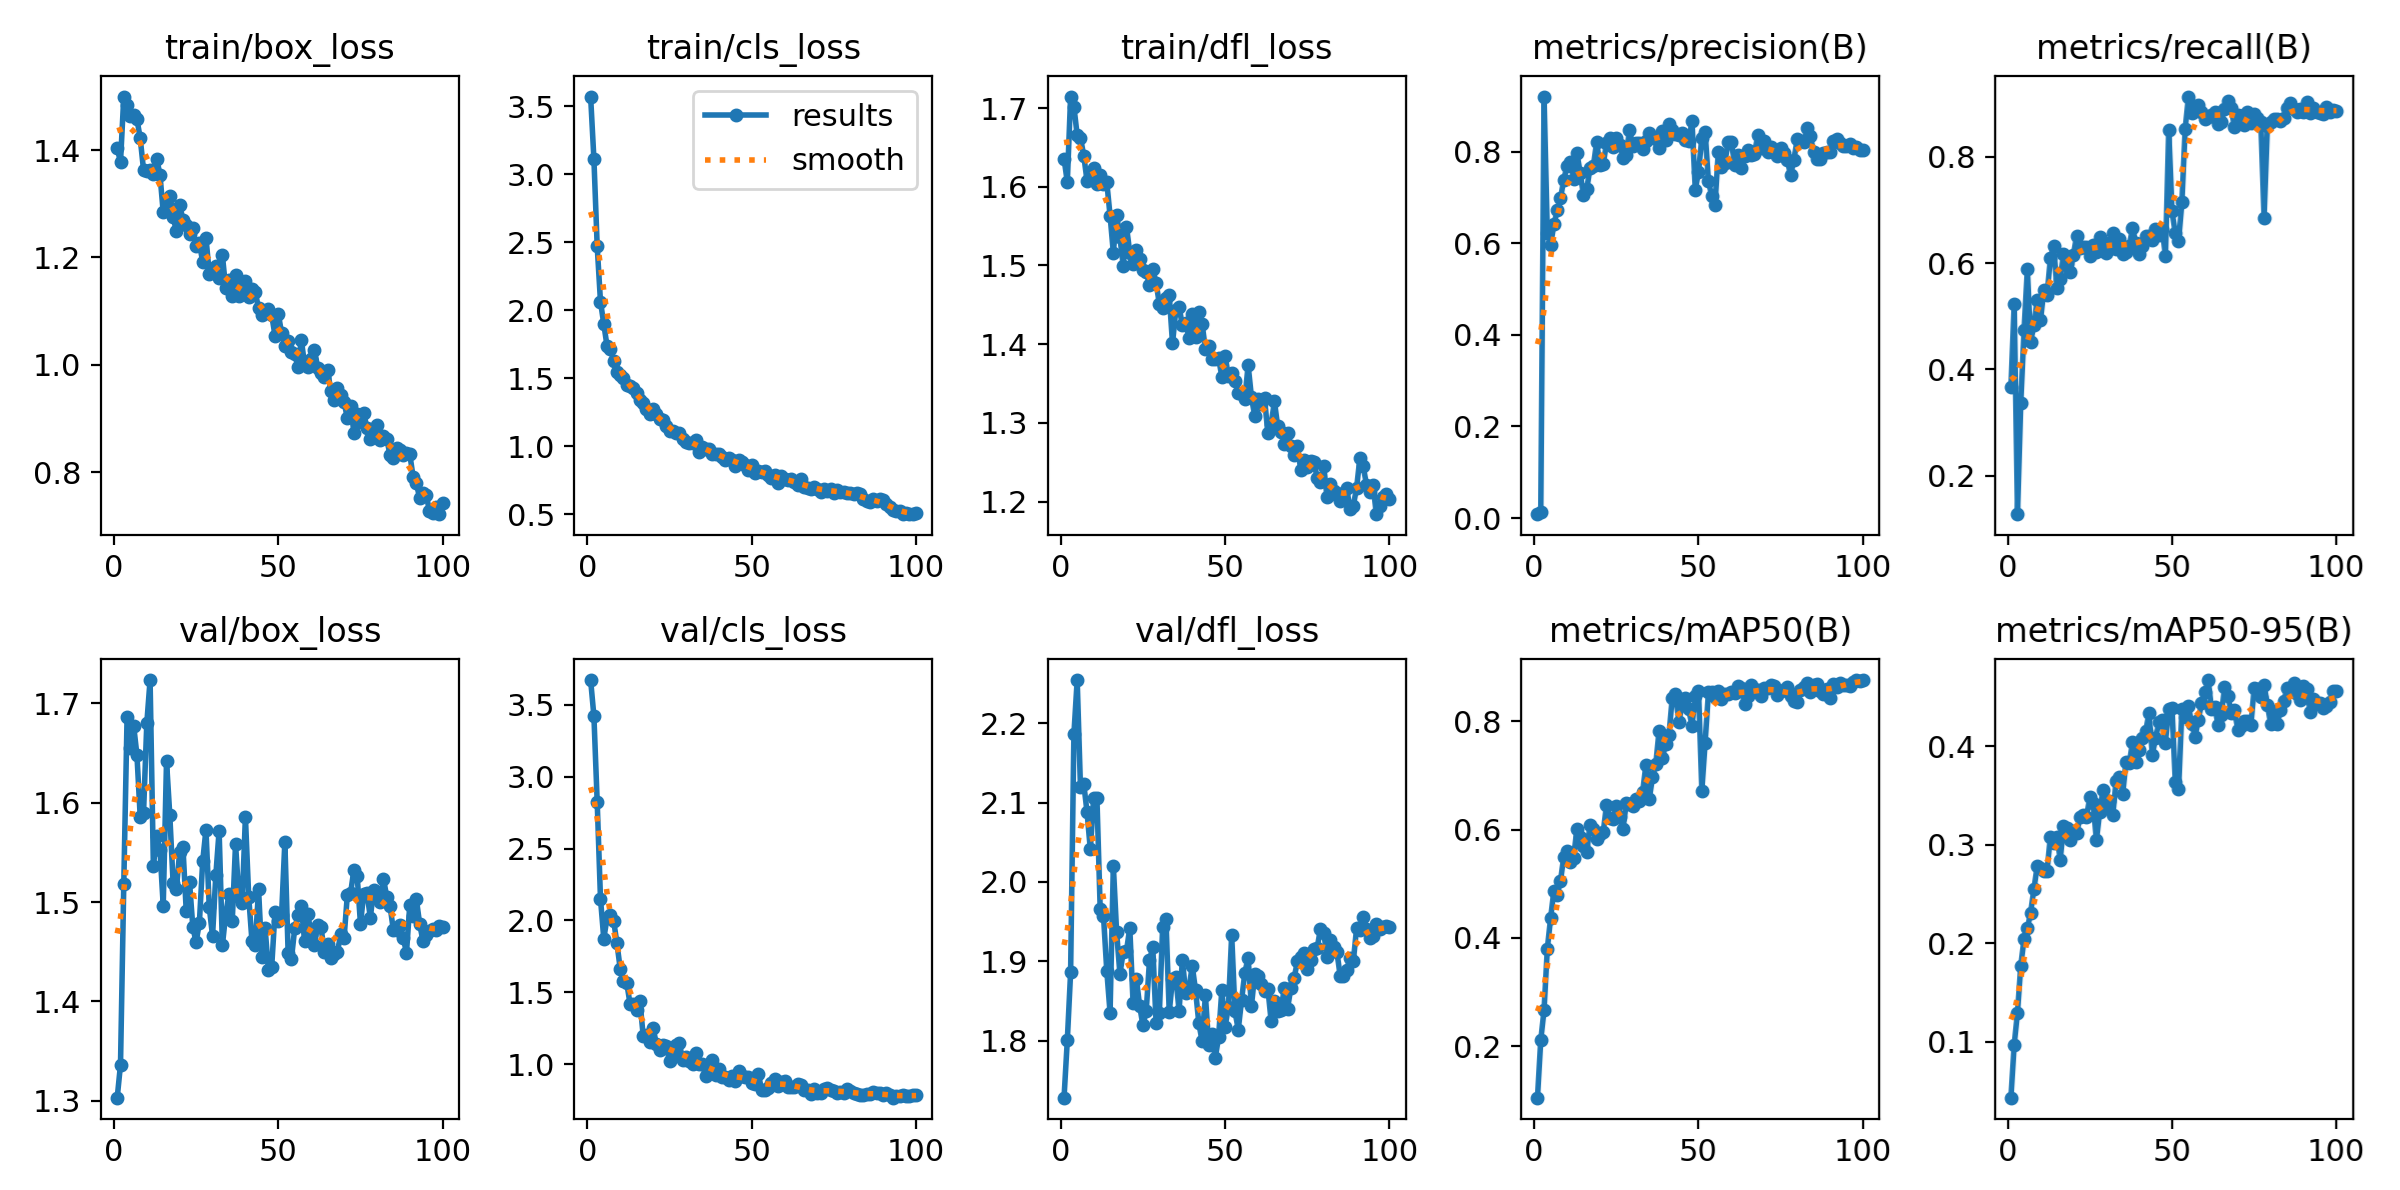
\includegraphics[width=1\linewidth]{Images/yolo11n_accuracy.png}
% %     \caption{Accuracy metrics of the original YOLO11n model}
% %     \label{fig:yolo11n_accuracy}
% % \end{figure}

% % \begin{figure}[ht]
% %     \centering
% %     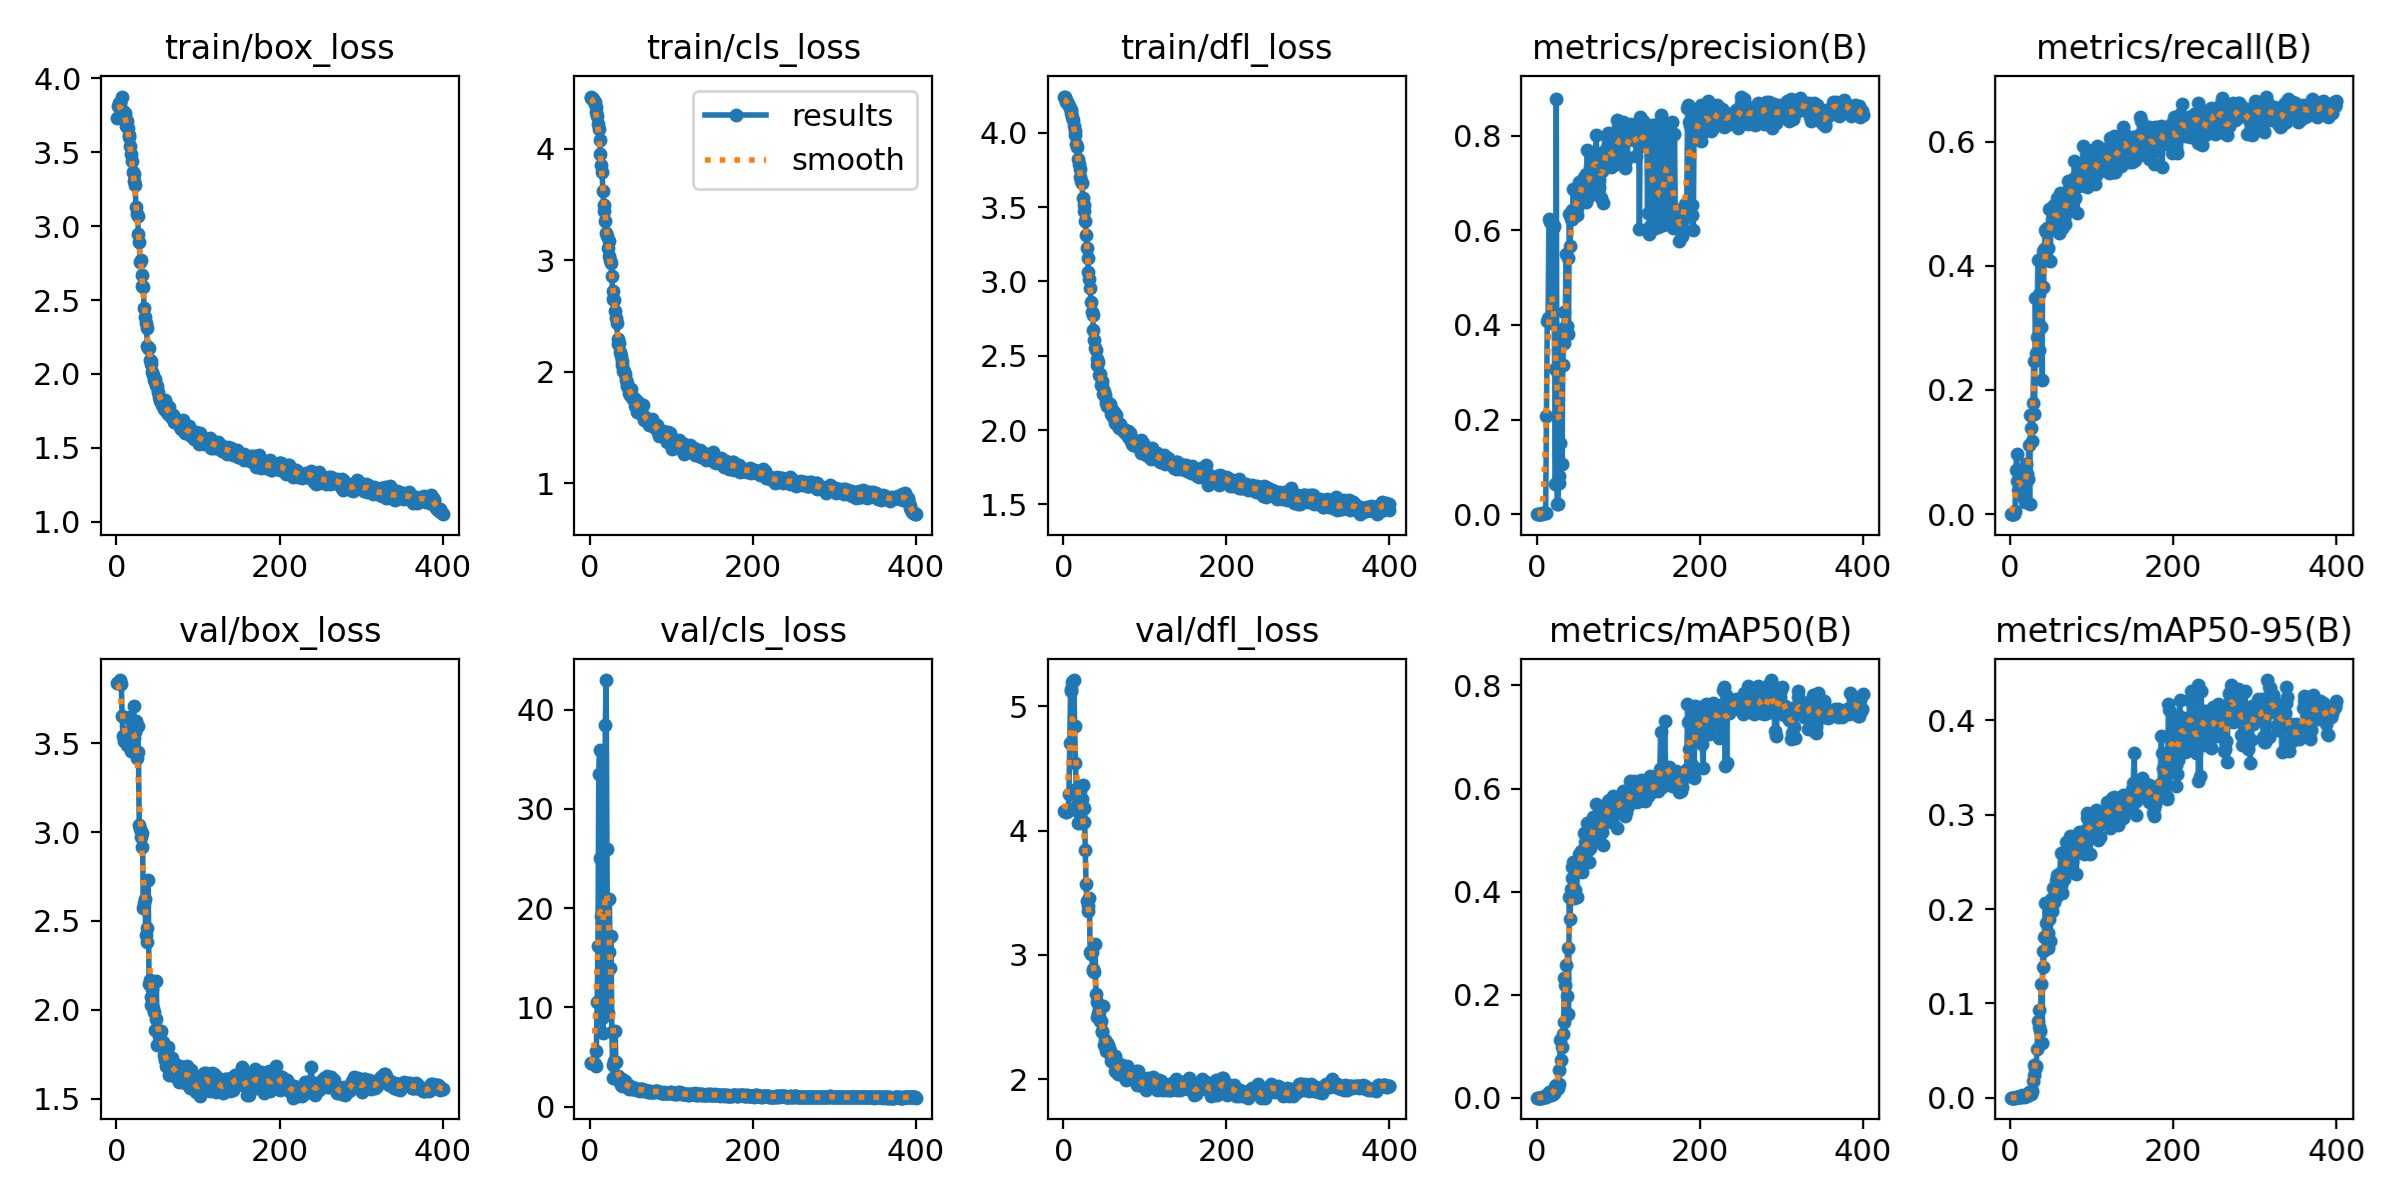
\includegraphics[width=1\linewidth]{Images/yolo11n-mbnv4accuracy.png}
% %     \caption{Accuracy metrics of YOLO11n--MobileNetV4 (ConvSmall)}
% %     \label{fig:yolo11n-mbnv4_accuracy}
% % \end{figure}


% Figures~\ref{fig:yolo11n_accuracy} and \ref{fig:yolo11n-mbnv4_accuracy} show that the original YOLO11n achieves higher detection accuracy, exceeding the MobileNetV4 variant by approximately 10--15\% in both mAP@50 and mAP@50--95. Despite this reduction, the MobileNetV4-based model retains over 85\% of the baseline accuracy, demonstrating stable convergence and sufficient detection performance for traffic light recognition.

% % Figures \ref{fig:compare-model} shows that the original YOLO11n achieves higher detection accuracy, exceeding the MobileNetV4 variant by approximately 10--15\% in both mAP@50 and mAP@50--95. Despite this reduction, the MobileNetV4-based model retains over 85\% of the baseline accuracy, demonstrating stable convergence and sufficient detection performance for traffic light recognition.


% \subsubsection{Inference Speed}

% Inference latency is the primary bottleneck for CPU-based edge deployment. According to official benchmarks, the original YOLO11n (TFLite) requires more than 400\,ms per frame on CPU, resulting in a throughput of only 2--3 FPS \cite{ultralytics_rpi5}.

% In contrast, as summarized in Table~\ref{tab:tradeoff_yolo_models}, the YOLO11n--MobileNetV4 model reduces inference latency to 30--40\,ms, corresponding to a 90--92\% reduction and a 10--13$\times$ speedup. This enables real-time performance of 25--33 FPS on embedded hardware, as illustrated in Fig.~\ref{fig:res_cpp}. The significant latency reduction validates the suitability of the MobileNetV4 backbone for real-time edge inference.

% \begin{table}[ht]
% \centering
% \caption{Performance trade-off between Different Models}
% \label{tab:tradeoff_yolo_models}
% \resizebox{\columnwidth}{!}{
% \renewcommand{\arraystretch}{1.3}
% \begin{tabular}{|l|l|c|c|c|l|}
% \hline
% Model & Format & Epochs & mAP@50 & mAP@50-95 & Inference time \\ \hline
% YOLO11n & liteRT & 100 & 0.977 & 0.785 & $\sim$90ms \\ \hline
% YOLO11-MobilenetV4 & liteRT & 400 & 0.755 & 0.443 & $\sim$36ms \\ \hline
% YOLO8n & liteRT & 100 & 0.974 & 0.811 & $\sim$78ms \\ \hline
% YOLO26n & liteRT & 100 & 0.978 & 0.821 & $\sim$55ms \\ \hline
% SSD-MobilenetV3 & ONNX & 100 & 0.743 & 0.548 & $\sim$40ms \\ \hline
% \end{tabular}
% }
% \end{table}

% The experimental results demonstrate the feasibility and efficiency of the proposed approach for real-time traffic light detection on edge devices. Based on these findings, the final section summarizes the key contributions and discusses the implications for future AUTOSAR-based edge perception systems.
